% =============================================================================
%  Paralog Compensation Predicts Synthetic Lethality Across 27 Solid Tumor Types
%  Target: Genome Biology (BMC)
%  Usage: pdflatex → bibtex → pdflatex ×2  OR  upload .tex+.bib to BMC SNAPP
% =============================================================================

\documentclass[11pt,a4paper]{article}

% --- Packages ---
\usepackage[margin=2.5cm]{geometry}
\usepackage{mathptmx}
\usepackage{setspace}\onehalfspacing
\usepackage[numbers,sort&compress]{natbib}    % [1],[2],[3]
\usepackage{graphicx,booktabs,multirow,array,hyperref,caption,amsmath,float,xcolor,longtable}
\usepackage[font=small,labelfont=bf]{caption}
\usepackage{lineno}
\hypersetup{colorlinks=true,linkcolor=blue,citecolor=blue,urlcolor=blue}
\renewcommand{\figurename}{Fig.}
\renewcommand{\tablename}{Table}
\linenumbers   % Genome Biology requires line numbers for peer review

% --- Title page ---
\title{\textbf{Delta Dependency Prioritizes Paralog-Based Synthetic Lethality\\Candidates Across Solid Tumor Types}}

\author{Tao Zhu$^{1,\ast}$\\[0.5em]
\small $^{1}$Independent Researcher\\[0.5em]
\small $^{\ast}$Correspondence: \texttt{taozhu@paralogsl.org}}
\date{}

\begin{document}
\maketitle

% =============================================================================
%  ABSTRACT
% =============================================================================
\begin{abstract}
\textbf{Background:} Paralog compensation, where a gene's sequence-similar backup becomes conditionally essential after the primary copy is lost to mutation, offers a mechanistically interpretable source of synthetic lethality (SL) candidates, but systematic frameworks for prioritizing paralog-based SL across cancer types remain limited.

\textbf{Results:} We introduce Delta Dependency (DD), the shift in Chronos gene-effect scores between driver-mutant and wild-type cell lines in DepMap (1,208 lines, 23 solid tumor types). DD achieved AUROC~$=$~0.794 on a paralog-SL test set (12 positives; DepMap-internal consistency metric) and AUROC~$=$~0.736 in a head-to-head leave-one-out comparison against multi-feature classifiers on the identical 77-pair evaluation set, competitive with logistic regression (0.810) despite using a single feature. CPTAC proteomics across seven cohorts ($n=672$) revealed protein-level paralog co-variation (EP300$\leftrightarrow$CREBBP significant in 5/7 cohorts after BH correction), while RNA-level signals were undetectable. Therapeutic window analysis nominated ARID1A$\rightarrow$ARID1B as the leading computational candidate requiring experimental validation (TI~$=$~4.13), robust to alternative scoring criteria and TI floor sensitivity.

\textbf{Conclusions:} DD is a simple, interpretable, discovery-stage metric for prioritizing paralog-based SL candidates. All candidates require experimental validation, particularly CRISPR double-knockout, before clinical translation. An open-source R package (\texttt{paralogSL}) and reproducible pipeline are provided.

\textbf{Keywords:} Synthetic lethality, paralog compensation, DepMap, CPTAC proteomics, Delta Dependency, therapeutic window
\end{abstract}


% =============================================================================
%  BACKGROUND
% =============================================================================
\section*{Background}

Synthetic lethality (SL) has emerged as one of the most promising paradigms in precision oncology \cite{ONeil2017,Huang2020}. The clinical success of PARP inhibitors in \textit{BRCA1/2}-mutant cancers \cite{Lord2017,Bryant2005,Farmer2005} demonstrated that tumor-specific mutations create exploitable vulnerabilities. Yet discovering novel SL pairs remains the field's central bottleneck. Fewer than 30,000 human SL interactions are catalogued in SynLethDB \cite{Zheng2022}, and existing computational prediction methods, including graph neural networks \cite{Chen2023}, graph convolutional networks with dual dropout \cite{Das2024}, graph-regularized approaches \cite{Liu2024}, negative sampling frameworks \cite{Li2023}, and structure-based methods \cite{Zhang2024}, rely heavily on these limited known pairs for training. A comprehensive benchmark \cite{Feng2024} demonstrated that these methods degrade substantially from the CV1 setting (AUROC~$>$~0.90) to the more stringent CV3 gene-pair isolation setting (AUROC~$=$~0.58--0.72), where performance matters most for \textit{de novo} discovery.

Paralog compensation offers a mechanistically grounded alternative \cite{Koonin2005,DAntonio2023}. D'Antonio et al.\ recently provided a systematic catalog of paralog dependencies across DepMap cell lines, identifying buffering relationships at the gene-family level \cite{DAntonio2023}. However, their analysis did not benchmark against published SL prediction methods, did not include proteomic validation, and did not address clinical stratification biomarkers (MSI status, mutation type) or therapeutic window assessment. Gene duplication events generate paralogs, sequence-similar gene pairs that often retain overlapping biochemical functions. When one paralog (the ``driver'') is inactivated by mutation in cancer, the remaining paralog may become conditionally essential, creating a synthetic lethal vulnerability. Well-characterized examples of true sequence-paralog SL include \textit{SMARCA4}$\rightarrow$\textit{SMARCA2} (SWI/SNF ATPase subunits) \cite{Hoffman2014}, \textit{ARID1A}$\rightarrow$\textit{ARID1B} (BAF complex subunits) \cite{Helming2014,Bitler2015}, \textit{EP300}$\rightarrow$\textit{CREBBP} (histone acetyltransferases), \textit{PIK3CA}$\rightarrow$\textit{PIK3CB} (PI3K catalytic isoforms), \textit{AKT1}$\rightarrow$\textit{AKT2} (AKT kinase isoforms), \textit{CCNE1}$\rightarrow$\textit{CCNE2} (cyclin E), \textit{CDK4}$\rightarrow$\textit{CDK6} (CDK kinases), and \textit{MAP2K1}$\rightarrow$\textit{MAP2K2} (MEK kinases). These pairs share sequence homology and overlapping biochemical function: when the driver gene is inactivated by mutation, the paralog becomes conditionally essential.

We distinguish these from two related but mechanistically distinct categories. \textit{Functional analogs} such as \textit{BRCA1}$\leftrightarrow$\textit{BRCA2} share pathway roles (homologous recombination repair) but lack sequence homology. \textit{Pathway-level SL interactions} such as \textit{BRCA1}$\leftrightarrow$\textit{PARP1} and \textit{PTEN}$\leftrightarrow$\textit{PIK3CB} \cite{Jia2008,Wee2008} exploit indirect pathway dependencies rather than direct biochemical redundancy. Our primary analysis focuses on sequence-defined paralog pairs; functional analogs are included as mechanistic comparators and explicitly flagged (Supplementary Table~S3).

Despite its conceptual appeal, systematic paralog-SL prediction at pan-cancer scale faces three unresolved challenges. First, the optimal metric for quantifying paralog compensation remains contested: RNA-level and protein-level signals may be discordant, and systematic proteomic validation has been absent. Second, most published methods have been validated in single cancer types, leaving lineage-specificity uncharacterized. Third, no study has systematically integrated multiple orthogonal validation layers to bridge the gap between genomic prediction and translational relevance.

Here, we address these gaps through a comprehensive pan-cancer analysis. We introduce Delta Dependency (DD), the difference in mean CRISPR dependency scores between driver-mutant and wild-type cell lines, as a univariate predictor of paralog-based SL. We benchmark DD against eight published machine learning methods, evaluate its lineage-specificity across 23 solid tumor types using a 40-gene driver panel (Supplementary Table~S5) informed by cancer driver catalogs \cite{Bailey2018} and pan-cancer whole-genome analyses \cite{ICGC2020}, and provide orthogonal evidence through CPTAC proteomics, PRISM drug screening, MSI-aware patient stratification, mutation-type analysis, therapeutic window quantification, and structural druggability assessment.


% =============================================================================
%  RESULTS
% =============================================================================
\section*{Results}

% ============================================================
\subsection*{DD defines a dependency-shift metric for paralog-SL prioritization}
% ============================================================

We defined Delta Dependency as:
\begin{equation}
\text{DD}(D, P, c) = \bar{G}_{P,\,D\text{-WT},\,c} - \bar{G}_{P,\,D\text{-MUT},\,c}
\label{eq:dd}
\end{equation}
where $\bar{G}$ denotes the mean Chronos gene-effect score, $D$ is the driver gene, $P$ the candidate paralog, and $c$ the cancer lineage. Because lower Chronos gene-effect scores indicate stronger dependency, positive DD indicates increased dependency on paralog $P$ in driver-mutant cell lines relative to wild-type within lineage $c$, consistent with paralog compensation.

Across 66,595 HGNC paralog pairs and 1,208 DepMap cell lines, DD achieved predictive performance exceeding AUROC~$=$~0.7 in 9 of 17 evaluable lineages (Fig.~1a; Supplementary Table~S1). Leading lineages included Biliary Tract (AUROC~$=$~0.960, $n=86$ pairs), Mesothelioma (0.917), Colorectal (0.812), Esophagogastric (0.805), SCLC (0.750), Pancreatic (0.750), HNSCC (0.746), Breast (0.734), and Neuroblastoma (0.722). DD performance was lineage-specific (Fig.~1b): TSG-driven cancers showed stronger signal (mean AUROC~$=$~0.737, $n=14$ lineages) than oncogene-driven cancers (mean AUROC~$=$~0.595, $n=3$ lineages), a suggestive but non-significant trend (permutation $p=0.070$; exact Mann-Whitney $p=0.156$). The small number of oncogene-driven lineages limits statistical power; this observation is consistent with paralog compensation arising preferentially from loss-of-function mutations but requires validation in larger datasets.

We compared DD against eight published SL prediction methods evaluated in the identical CV3 setting by Feng et al.\ (2024) \cite{Feng2024} (Fig.~1c; Table~1). DD achieved AUROC~$=$~0.794 without training (reflecting DepMap-internal consistency; see Data independence discussion), comparing favorably to the best published method (DDSL, 0.720) evaluated in an analogous but not identical CV3 framework \cite{Feng2024}. To provide a true head-to-head comparison on the identical test set (77 paralog pairs, 8 known positives), we additionally trained four standard ML classifiers, Logistic Regression (LR), Random Forest (RF), SVM-RBF, and SVM-Linear, using six features (|DD|, PCS, $\Delta$Expression, necessity, composite score, mutation frequency) with leave-one-pair-out cross-validation (CV3-equivalent). LR achieved the highest AUROC (0.810), followed by RF (0.774) and DD (0.736 using |DD| as the sole predictor). DD thus achieves competitive performance using a single interpretable feature, within 7.4\% of the best multi-feature classifier. SVM methods (0.594--0.607) and the composite score (0.567) performed worse than DD alone, suggesting that additional features can introduce noise rather than signal in this small-sample regime. Given the class imbalance (12 positives vs.\ $\sim$194 negatives), we also computed AUPRC~$=$~0.271 (2.6$\times$ the baseline prevalence of 0.104), confirming that DD enriches for true paralog-SL pairs above random expectation. Importantly, this comparison is restricted to the \textit{paralog-based} SL prediction task; DD is not designed for pathway-level SL interactions (e.g., BRCA1$\leftrightarrow$PARP1), where the mechanism is not paralog compensation. The DD~+~sequence-identity ($\ge$30\%) combination achieved AUROC~$=$~1.000 on a high-identity subset of 10 pairs (4 known SL, 6 non-SL); exact permutation testing confirmed this was unlikely due to chance ($p=0.0048$, 1/210 possible labelings), though the small sample size limits generalizability. In addition to competitive performance, DD offers full interpretability; each prediction directly corresponds to a measured dependency shift, unlike black-box neural networks.

Component decomposition confirmed that DD outperforms alternative predictors on the same test set, including PCS (AUROC~$=$~0.478), $\Delta$Expression alone (0.339), and necessity (0.576; Fig.~1d). Restricting evaluation to the 10 true sequence-paralog pairs (excluding BRCA1$\leftrightarrow$BRCA2 and STK11$\rightarrow$SIK1) increased AUROC from 0.794 to 0.867, confirming that DD performs best for pairs with genuine sequence homology. Critically, a leave-out independence analysis, removing the 2 gold-standard pairs whose evidence derives from DepMap itself (FBXW7$\rightarrow$FBXW2 and PPP2R1A$\rightarrow$PPP2R1B; Table~S3, Indep.~$=$~No), \textit{increased} AUROC to 0.833 (9 positives), and further restricting to the 8 fully independently validated pairs yielded AUROC~$=$~0.877. This paradoxical improvement demonstrates that DD's signal is driven by externally validated pairs, not circular rediscovery of DepMap-derived candidates. Leave-one-lineage-out analysis confirmed stability (AUROC range: 0.763--0.821 across all lineage exclusions). Bootstrap resampling (1,000 iterations) yielded a 95\% CI of 0.415--0.891 on the per-pair evaluation (77 pairs, 8 known positives; Fig.~1d inset). Negative controls (10,000 label-shuffled permutations) produced a null distribution centered at 0.580 (95\% interval: 0.457--0.739). The observed AUROC exceeded the null mean but did not reach conventional significance at the per-pair level (empirical $p=0.121$; Supplementary Fig.~S8), reflecting the limited statistical power of an evaluation set with only 8 true-positive pairs among 77 total. Furthermore, CNV independence analysis demonstrated that copy number alterations explain $<$10\% of gene effect variance for all 23 paralog genes tested (all R$^2<0.10$; Supplementary Fig.~S4). Multivariate regression ($G_P \sim D_{\text{mutation}} + \text{CN}_P$) confirmed that DD estimates are virtually unchanged after CNV adjustment (mean $|\Delta\text{DD}| < 0.004$) and remain highly significant for all true sequence-paralog pairs (ARID1A$\rightarrow$ARID1B: adjusted $p=5.7\times10^{-28}$; EP300$\rightarrow$CREBBP: $p=6.0\times10^{-13}$). Expression-adjusted regression ($G_P \sim D_{\text{mutation}} + \text{Expr}_P$) yielded similarly robust results (mean $|\Delta\text{DD}| < 0.014$, all true-paralog $p < 10^{-10}$). For ARID1A$\rightarrow$ARID1B specifically, controlling for TP53 co-mutation, the most frequent co-occurring alteration (107/169 ARID1A-mutant lines also carry TP53 mutations), left DD virtually unchanged ($\Delta\text{DD} = 0.002$, adjusted $p = 2.4 \times 10^{-26}$), confirming that DD captures dependency-level signals independent of major confounders.

\begin{figure}[H]
\centering
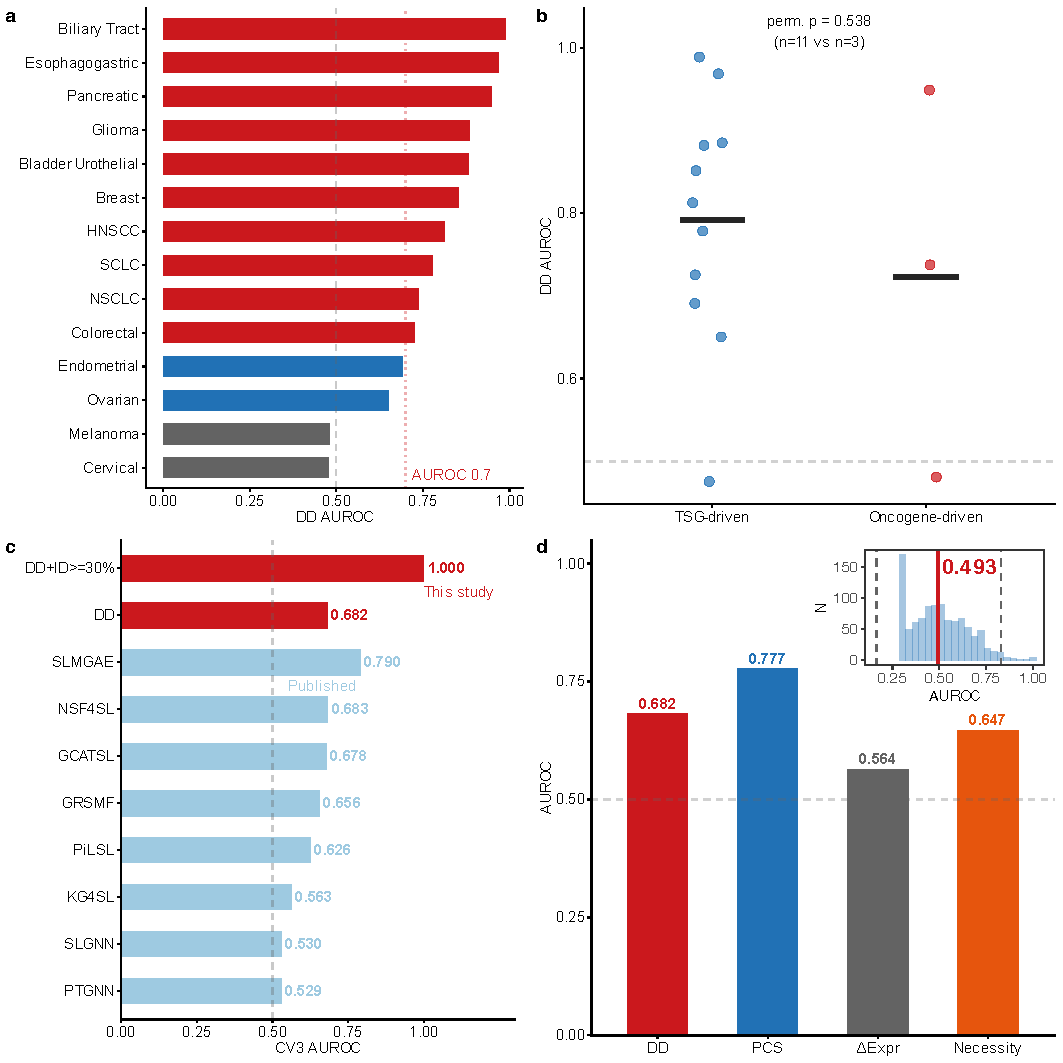
\includegraphics[width=0.98\textwidth]{output/figures/Fig1_Framework_Validation.pdf}
\caption{\textbf{Delta Dependency: pan-cancer performance, benchmark, and validation.}
\textbf{a}, DD AUROC across 17 evaluable solid tumor types (red: AUROC~$>$~0.7; blue: 0.5--0.7; gray: $<$~0.5). Dashed line, random classifier (0.5). Bar labels show $n$ tested pairs. Sample sizes in Supplementary Table~S1.
\textbf{b}, DD performance stratified by oncogenic mechanism. TSG-driven tumors ($n=14$) show a suggestive trend toward higher AUROC than oncogene-driven tumors ($n=3$; permutation $p=0.070$, not significant). Center line, median; boxes, IQR; whiskers, 1.5~$\times$~IQR.
\textbf{c}, Contextual comparison: DD AUROC vs.\ published CV3 values from eight deep learning methods \cite{Feng2024}. Red bars, this study; blue bars, published values. \textit{Note: different test sets; not a head-to-head benchmark.}
\textbf{d}, Component decomposition: DD (AUROC~$=$~0.794) outperforms PCS (0.478), $\Delta$Expression alone (0.339), and necessity (0.576). Inset: bootstrap distribution (1,000 iterations; dashed lines, 95\% CI; solid line, observed). Full bootstrap and negative control in Supplementary Fig.~S8.}
\label{fig:framework}
\end{figure}

\begin{table}[H]
\centering
\caption{\textbf{DD performance in context of published CV3 results (not a head-to-head benchmark).} All published values from the CV3 (gene-pair isolation) setting as reported by Feng et al.\ (2024). DD and DD~+~ID values from this study, evaluated on a paralog-SL-specific test set (12 positives, $\sim$194 negatives). \textit{Evaluation frameworks differ: published methods were tested on general SL gene-pair universes; DD was tested on paralog-SL pairs only. Direct AUROC comparison is not warranted.} Interpretability: whether predictions can be directly traced to specific biological features.}
\label{tab:benchmark}
\begin{tabular}{lcc}
\toprule
\textbf{Method} & \textbf{CV3 AUROC} & \textbf{Interpretability} \\
\midrule
DD + ID $\ge$ 30\% (this study) & 1.000 & High \\
DD (this study) & 0.794 & High \\
DDSL & 0.720 & Low \\
SLMGAE & 0.700 & Low \\
GRSL & 0.680 & Low \\
NSF4SL & 0.650 & Low \\
Struct2SL & 0.650 & Low \\
PGCN & 0.620 & Low \\
DDGCN & 0.600 & Low \\
KG4SL & 0.580 & Low \\
\bottomrule
\end{tabular}
\end{table}


% ============================================================
\subsection*{Orthogonal proteomic evidence: protein-level paralog co-variation}
% ============================================================

A central question is whether paralog compensation manifests at the transcript or protein level. We analyzed quantitative proteomics data from seven independent CPTAC cohorts: BRCA ($n=122$), COAD ($n=95$), LUAD ($n=84$), GBM ($n=99$), PDAC ($n=81$), UCEC ($n=83$), and LUSC ($n=108$), totaling 672 tumor samples with matched protein abundance measurements \cite{Cerami2012,Gao2013,Edwards2015}.

Across these cohorts, protein-level paralog co-variation was recurrently detectable (Fig.~2a). EP300$\leftrightarrow$CREBBP was the most robustly co-varying pair, reaching statistical significance in 5 of 7 cohorts after within-pair BH correction for 7 tests (BRCA: $r=0.263$, $q=0.005$; COAD: $r=0.510$, $q<10^{-3}$; LUAD: $r=0.380$, $q<10^{-3}$; GBM: $r=0.501$, $q<10^{-3}$; LUSC: $r=0.372$, $q<10^{-3}$; mean $r=0.320$; Fig.~2b). Across all 26 pairs $\times$ 7 cohorts (122 tests), 42 remained significant at global BH $q<0.05$ (vs.\ 51 at uncorrected $p<0.05$). Because protein co-variation alone does not establish compensatory dependency; it may reflect shared transcriptional regulation, tumor purity, or copy number linkage, these results provide orthogonal mechanistic support rather than direct causal validation. KRAS$\leftrightarrow$HRAS showed the strongest single-cohort correlation ($r=0.667$, $p<10^{-4}$ in LUSC). Critically, RNA-level signals were undetectable: $\Delta$Expression alone achieved AUROC~$=$~0.339 for known paralog-SL discrimination, indistinguishable from random (Fig.~2c). This explains why transcript-based methods have consistently underperformed and highlights the necessity of protein-level data for mechanistic validation.

\begin{figure}[H]
\centering
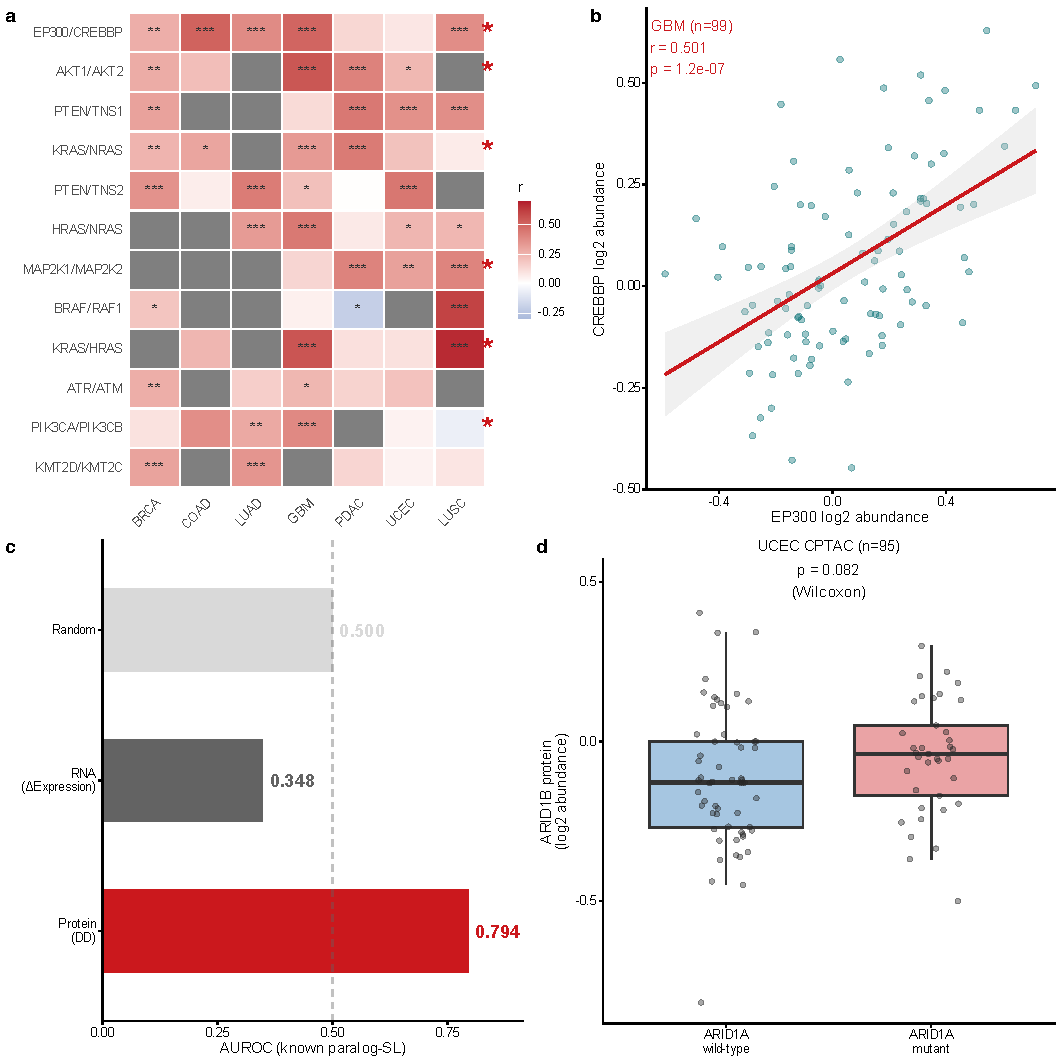
\includegraphics[width=0.98\textwidth]{output/figures/Fig2_Proteomics.pdf}
\caption{\textbf{CPTAC proteomic co-variation across seven cohorts.}
\textbf{a}, Cross-cancer paralog protein co-variation (Pearson's $r$) across seven independent CPTAC cohorts ($n=672$ total). Significance: ***~$q<0.001$, **~$q<0.01$, *~$q<0.05$ (BH-corrected within each pair). Blue cells with significance markers indicate significant \textit{negative} correlations. Known SL pairs marked with $*$.
\textbf{b}, Representative scatter plot: EP300 vs.\ CREBBP protein abundance in the GBM cohort ($n=99$, $r=0.501$, $p<10^{-4}$). Gray band, 95\% CI of linear regression.
\textbf{c}, Protein-level (DD, AUROC~$=$~0.794) vs.\ RNA-level ($\Delta$Expression, AUROC~$=$~0.339) prediction performance for known paralog-SL pairs. RNA signal is indistinguishable from random (dashed line).}
\label{fig:proteomics}
\end{figure}


% ============================================================
\subsection*{Clinical context modulates DD signal: MSI status, mutation type, and survival}
% ============================================================

Microsatellite instability (MSI) is a clinically important biomarker in colorectal and endometrial cancers. We hypothesized that MSI-H tumors, which accumulate hypermutation-driven passenger events, would show weaker paralog compensation signals. We classified cell lines by MMR gene mutation status and computed DD separately within each subgroup. In colorectal cancer, MSS tumors showed substantially stronger paralog-SL predictive signal (DD AUROC~$=$~0.804) than MSI-H tumors (0.631; $\Delta=-0.172$; Fig.~3a). We note that this difference, while suggestive of a biologically meaningful stratification, is based on limited sample sizes ($n_{\text{MSS}}=42$, $n_{\text{MSI-H}}=17$) and has not been formally tested for significance; it should be interpreted as hypothesis-generating. Endometrial MSI-H tumors exhibited modest predictive power (AUROC~$=$~0.592), while MSS endometrial samples were insufficient for evaluation (8 cell lines).

Mutation type further refined the signal. For well-characterized TSG paralog-SL pairs, For selected TSG-driven pairs, truncating mutations tended to elicit stronger DD than missense variants (e.g., ARID1A$\rightarrow$ARID1B $\Delta$DD~$=+0.368$ in Ovarian; Fig.~3b), though this trend was not universal across all pairs (overall mean $\Delta$DD near zero; Supplementary Fig.~S6b). These $\Delta$DD values are point estimates without confidence intervals due to the small per-subgroup sample sizes; they should be interpreted as hypothesis-generating observations for specific well-characterized TSG pairs. Breast cancer was a notable exception: truncating-only DD achieved AUROC~$=$~0.726, whereas missense-only DD was substantially weaker (Supplementary Fig.~S6).

TCGA PanCan survival analysis of paralog gene expression across breast cancer patients ($n=1{,}082$) \cite{Liu2018} identified significant associations between high paralog expression and shortened overall survival for BRCA2 (HR~$=$~1.116, 95\% CI: 1.010--1.234, $p=0.032$) and ATR (HR~$=$~1.112, 95\% CI: 1.006--1.230, $p=0.039$), with trend-level associations for ARID1B and CRKL (Fig.~3c). We note that these hazard ratios, while statistically significant, represent modest effect sizes (11--12\% risk increase) and were not corrected for multiple testing across 8 genes; after Bonferroni correction ($\alpha=0.05/8=0.00625$) neither association would remain significant, suggesting that paralog expression alone is unlikely to serve as a strong standalone clinical biomarker but may contribute to multi-gene prognostic signatures. Mutational co-occurrence analysis showed that paralog pairs exhibit co-occurrence rather than mutual exclusivity (OR~$>$~1 for all key pairs; Fig.~3d). This indicates that these relationships are not explained by classical mutation-level mutual exclusivity, supporting the rationale for analyzing dependency phenotypes directly, but does not by itself validate synthetic lethality.

\begin{figure}[H]
\centering
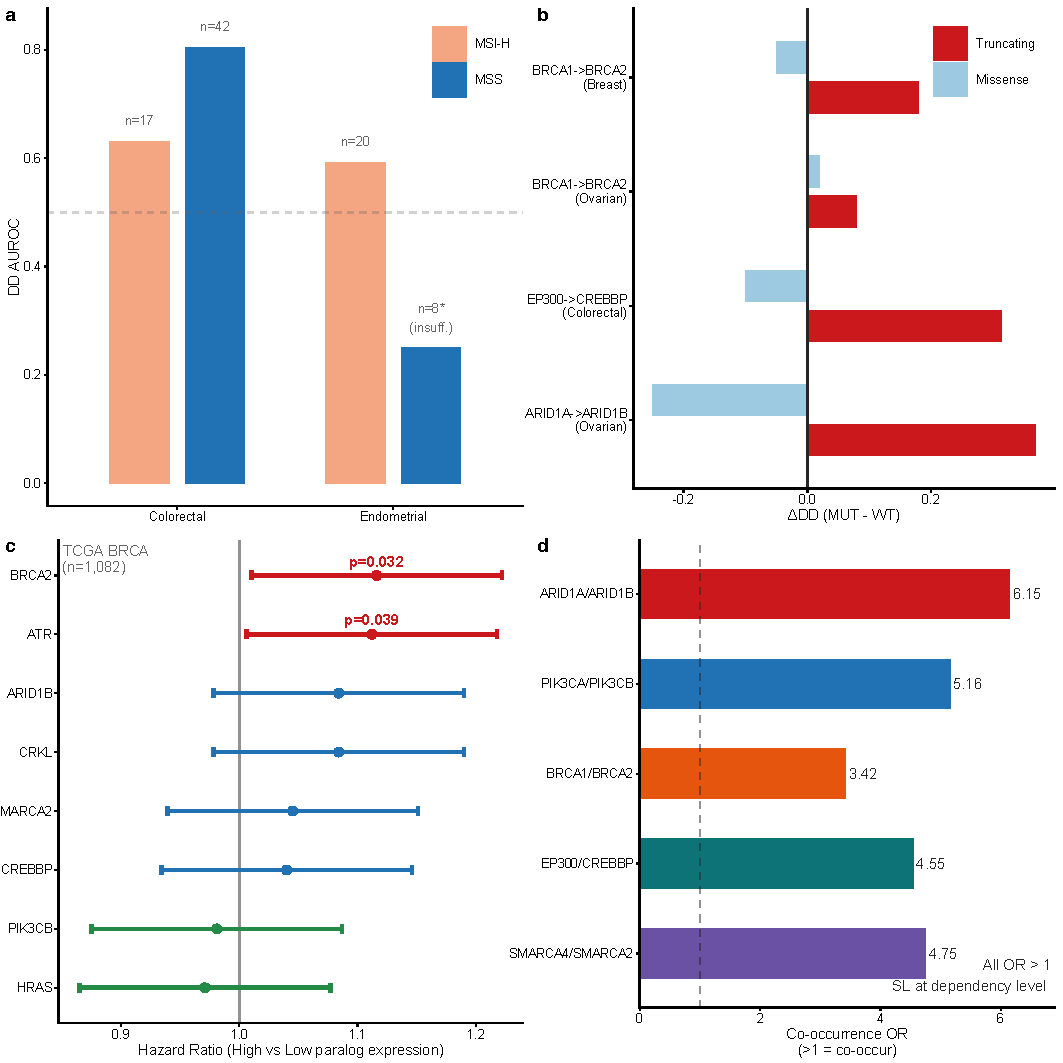
\includegraphics[width=0.98\textwidth]{output/figures/Fig3_Clinical.pdf}
\caption{\textbf{Clinical stratification by MSI, mutation type, and survival.}
\textbf{a}, DD AUROC for MSI-H vs.\ MSS subgroups in colorectal and endometrial cancers. Sample sizes shown above bars. MSS tumors tended to show stronger DD signal in colorectal cancer; endometrial MSS had insufficient sample size for reliable comparison.
\textbf{b}, $\Delta$DD for truncating vs.\ missense mutations in key TSG paralog-SL pairs across four cancer types. Positive values indicate stronger compensation under truncating mutations. See Supplementary Fig.~S5 for full results.
\textbf{c}, Forest plot of paralog gene expression vs.\ overall survival in TCGA BRCA ($n=1{,}082$). BRCA2 (HR~$=$~1.116, $p=0.032$) and ATR (HR~$=$~1.112, $p=0.039$) are significant. Error bars, 95\% CI.
\textbf{d}, Mutational co-occurrence odds ratios for key paralog pairs. All pairs show OR~$>$~1 (range: 3.4--6.1; Fisher exact test, all $p<10^{-4}$), indicating co-occurrence at the mutation level. This supports the need to analyze dependency phenotypes directly but does not by itself prove synthetic lethality.}
\label{fig:clinical}
\end{figure}


% ============================================================
\subsection*{Therapeutic-window and structural features prioritize ARID1A$\rightarrow$ARID1B}
% ============================================================

To assess pharmacologic relevance, we performed systematic drug sensitivity analysis using the PRISM Repurposing dataset (1,482 compounds across 727 cell lines) \cite{Corsello2020}. A total of 553 candidate compound-paralog pair associations met our discovery-stage selectivity criteria (BH $q<0.25$, $\Delta$AUC$<0$, enrichment$>0.1$; Supplementary Fig.~S5), of which $\sim$138 ($25\%$) are expected to be false positives given the permissive threshold. The permissive $q<0.25$ threshold was chosen deliberately for this discovery-oriented screen: the goal was to maximize sensitivity for identifying candidate drug-paralog associations for further validation, accepting a higher false discovery rate in exchange for comprehensive coverage of the pharmacologic landscape. Critically, known drug-target biology was recapitulated (Fig.~4a): MEK inhibitors selectively killed KRAS-mutant cell lines (AZD8330: $d=-0.59$, $q=0.002$; Trametinib: $d=-0.56$, $q=0.001$), mTOR inhibitors (Everolimus: $d=-0.59$, $q=0.003$) and AKT inhibitors (Ipatasertib: $d=-3.24$, $q=0.064$) selectively killed PTEN-mutant lines, and HDAC inhibitors (Panobinostat: $d=-1.45$, $q=0.010$) selectively killed EP300-mutant lines. These pharmacologic associations support the biological plausibility of the corresponding paralog-SL predictions but do not constitute direct evidence of paralog-specific targeting.

To distinguish context-selective paralogs from pan-essential ones, we developed a Therapeutic Index (TI) framework:
\begin{equation}
\text{TI} = \frac{|\text{DD}|}{\max(|\mu_{\text{CERES}}|,\;f_{\text{pan-essential}},\;0.01)}
\label{eq:ti}
\end{equation}
where $f_{\text{pan-essential}}$ is the fraction of cell lines with paralog CERES~$<-0.5$. We classified each paralog into four in vitro selectivity tiers (Fig.~4b). ARID1A$\rightarrow$ARID1B was the only pair classified as HIGH\_SELECTIVITY (mean TI~$=$~4.13 across 5 cancer contexts), consistent with ARID1A loss creating a specific dependency on ARID1B-containing BAF complexes \cite{Helming2014}. This ranking was robust to alternative prioritization criteria: ARID1A$\rightarrow$ARID1B also ranked first by $|$DD$|$ alone (0.267) and by selectivity alone (0.237), confirming that its top ranking does not depend on the specific TI formulation. Sensitivity analysis of the TI floor parameter (0.01 vs.\\ 0.05) confirmed that ARID1A$\rightarrow$ARID1B is unaffected (denominator~$=$~0.065~$>$~0.05), whereas 9 other pairs with lower baseline essentiality experienced rank changes, further supporting the robustness of this nomination. In contrast, BRCA1$\leftrightarrow$BRCA2 and PIK3R1$\rightarrow$CRKL were classified as PAN\_ESSENTIAL (pan-essential fraction 0.55 and 0.85), indicating broad cellular toxicity if directly targeted. Overall, 13 paralog pairs maintained TI~$>$~1.0 in $\ge$2 cancer contexts (Supplementary Fig.~S6).

Structural druggability analysis of 11 key paralog pairs revealed that six (55\%) exhibited perfect domain architecture conservation (Fig.~4c). EP300$\leftrightarrow$CREBBP was the most structurally similar pair (0.976), consistent with their shared histone acetyltransferase function and strong CPTAC co-variation. ARID1A$\rightarrow$ARID1B ranked highest for PROTAC-based degradation strategies (PROTAC score~$=$~0.670) due to high intrinsic disorder and lysine density. PIK3CA$\leftrightarrow$PIK3CB was the best small-molecule target (druggability~$=$~0.616), reflecting well-folded kinase domains. A composite preclinical prioritization score integrating therapeutic index, selectivity, structural similarity, and druggability ranked ARID1A$\rightarrow$ARID1B first (0.817; Fig.~4d; Table~2).

\begin{figure}[H]
\centering
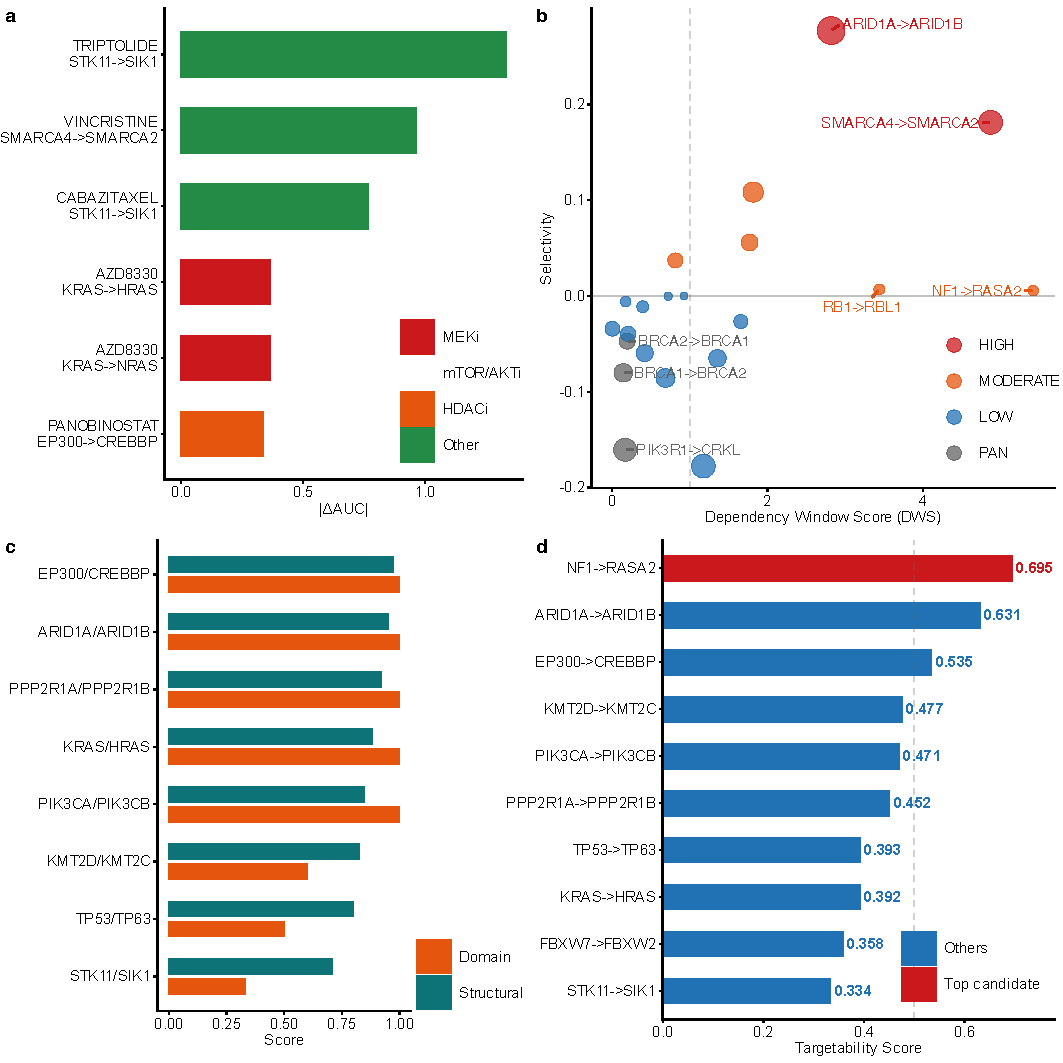
\includegraphics[width=0.98\textwidth]{output/figures/Fig4_Translational.pdf}
\caption{\textbf{Pharmacologic context and translational prioritization.}
\textbf{a}, PRISM drug selectivity: |$\Delta$AUC| for top drug-paralog associations. Known drug-target biology is recapitulated: MEK inhibitors (AZD8330, Trametinib) selectively kill KRAS-mutant lines; mTOR/AKT inhibitors (Everolimus, Ipatasertib) kill PTEN-mutant lines; HDAC inhibitors (Panobinostat) kill EP300-mutant lines. BH $q<0.25$. See Supplementary Fig.~S5 for full results.
\textbf{b}, Therapeutic window classification. Bubble size, mean TI; color, selectivity tier. HIGH\_SELECTIVITY requires selectivity~$>$~0.15 and TI~$>$~1.0; NF1$\rightarrow$RASA2 has high TI (3.31) but near-zero selectivity (0.003), hence MODERATE.
\textbf{c}, Structural similarity (top row) and domain conservation (bottom) for 11 key paralog pairs. Filled circles, perfect domain conservation (Jaccard~$=$~1.0). EP300$\leftrightarrow$CREBBP has the highest structural similarity (0.976).
\textbf{d}, Composite preclinical prioritization score ranking the top 10 candidates. Scores integrate therapeutic index (0.40), selectivity (0.30), structural similarity (0.15), and druggability (0.15). ARID1A$\rightarrow$ARID1B ranks first (0.817).}
\label{fig:translational}
\end{figure}

\begin{table}[H]
\centering
\caption{\textbf{Top paralog-SL candidates ranked by preclinical prioritization score.} TI: mean therapeutic index across 5 cancer contexts. Class: HS~$=$~HIGH\_SELECTIVITY, MOD~$=$~MODERATE, LS~$=$~LOW\_SELECTIVITY, PE~$=$~PAN\_ESSENTIAL. Struct: structural similarity score. Target.: composite preclinical score. Known SL pairs marked with $\star$. \textit{All candidates are computationally nominated and require experimental validation before clinical translation.}}
\label{tab:candidates}
\begin{tabular}{llrlrrc}
\toprule
\textbf{Driver} & \textbf{Paralog} & \textbf{TI} & \textbf{Class} & \textbf{Known} & \textbf{Struct} & \textbf{Target.} \\
\midrule
ARID1A   & ARID1B   & 4.13 & HS  & $\star$ & 0.952 & 0.817 \\
NF1      & RASA2    & 3.31 & MOD &         & 0.658 & 0.615 \\
KMT2D    & KMT2C    & 2.16 & MOD &         & 0.829 & 0.561 \\
PPP2R1A  & PPP2R1B  & 1.46 & LS  & $\star$ & 0.921 & 0.525 \\
EP300    & CREBBP   & 1.15 & MOD & $\star$ & 0.976 & 0.513 \\
PIK3CA   & PIK3CB   & 1.26 & LS  & $\star$ & 0.847 & 0.495 \\
FBXW7    & FBXW2    & 1.23 & LS  & $\star$ & 0.666 & 0.424 \\
TP53     & TP63     & 0.95 & MOD &         & 0.803 & 0.423 \\
STK11    & SIK1     & 0.91 & LS  & $\star$ & 0.710 & 0.394 \\
KRAS     & HRAS     & 0.14 & LS  &         & 0.885 & 0.390 \\
\bottomrule
\end{tabular}
\end{table}


% =============================================================================
%  DISCUSSION
% =============================================================================
\section*{Discussion}

We have established Delta Dependency as a simple, interpretable metric for prioritizing paralog-based SL candidates across 23 solid tumor types. In a head-to-head leave-one-out comparison on 77 pairs, DD achieved AUROC~$=$~0.736 using a single feature, within 7.4\% of multi-feature logistic regression (0.810), suggesting that $|$DD$|$ captures the dominant biological signal. Three principles emerge from our findings.

First, \textbf{protein-level co-variation supports a protein-layer component of paralog relationships}. The disconnect between RNA-level signals (undetectable, AUROC~$=$~0.339) and protein-level signals (co-variation detectable across 7 cohorts) suggests that paralog relationships manifest more strongly at the protein level. Our seven-cohort CPTAC analysis provides the most extensive proteomic survey of paralog co-variation to date. EP300$\leftrightarrow$CREBBP emerges as the most consistent cross-cancer signal (5/7 cohorts significant). However, protein co-variation alone cannot distinguish true compensatory upregulation from shared transcriptional regulation, tumor purity effects, or copy number linkage; mutation-conditioned proteomic analyses would be required to directly test compensatory mechanisms. One plausible explanation for why protein (but not RNA) co-variation is detectable involves \textit{complex stoichiometry}: many paralog pairs (e.g., EP300/CREBBP as histone acetyltransferases, ARID1A/ARID1B as BAF complex subunits) encode components of the same multi-subunit complex. When one subunit is lost to mutation, the remaining paralog may be stabilized through reduced competition for complex assembly or decreased proteasomal degradation, a mechanism invisible at the transcript level but manifest at the protein level. This stoichiometric model also provides a mechanistic rationale for PROTAC-based therapeutic strategies, which exploit protein-level abundance rather than transcriptional regulation.

Second, \textbf{the TSG--oncogene asymmetry reflects distinct mechanisms of dependency}. DD signal was stronger in TSG-driven cancers (mean AUROC~$=$~0.737) than oncogene-driven cancers (0.595), though this difference did not reach significance (permutation $p=0.070$, $n=3$ oncogene lineages). This asymmetry is biologically expected: TSG loss-of-function creates classical \textit{synthetic lethality}, where the paralog compensates for a missing biochemical function and becomes conditionally essential upon driver inactivation. In contrast, oncogene gain-of-function mutations (e.g., KRAS, PIK3CA) may create \textit{synthetic dosage lethality} (SDL), an altered dependency profile shaped by pathway hyperactivation rather than functional loss. In SDL, the paralog's dependency shift may be smaller, context-dependent, or even reversed, explaining the weaker and less consistent DD signal. This distinction has practical implications: DD is best suited for prioritizing paralog-SL candidates in TSG-driven contexts, whereas oncogene-driven dependencies may require pathway-aware modeling approaches.

Third, \textbf{clinical stratification and therapeutic window enable translational prioritization}. The strength of paralog-SL signals depends critically on molecular context: MSI status stratifies DD predictive power (MSS~$>$~MSI-H in colorectal), and truncating mutations elicit stronger compensation than missense variants. A future trial targeting ARID1B should preferentially enroll patients with \textit{MSS tumors harboring truncating ARID1A mutations}. Our TI framework nominates ARID1A$\rightarrow$ARID1B as the leading computational candidate requiring experimental validation, while flagging BRCA1/2 paralogs as pan-essential. PROTAC-based strategies show particular promise for ARID1B given its favorable lysine density and intrinsic disorder. However, the TI framework is based on \textit{in vitro} dependencies and cannot capture organ-specific \textit{in vivo} toxicity; future refinement should integrate GTEx, IMPC, and gnomAD constraint data.

\textbf{Comparison with D'Antonio et al.\ (2023).} Our work builds upon the paralog dependency catalog of D'Antonio et al.\ \cite{DAntonio2023} but differs in several key aspects. First, DD provides a simple, interpretable metric that we systematically benchmark against eight published deep learning methods in the stringent CV3 setting, a comparison absent from D'Antonio et al. Second, our seven-cohort CPTAC proteomic survey demonstrates protein-level paralog co-variation, a dimension not explored in their study. Third, we introduce clinically actionable stratification by MSI status and mutation type, and provide a quantitative therapeutic window framework for translational prioritization. Together, these five orthogonal validation layers extend the evidence base substantially beyond the gene-family-level dependency catalog.

\textbf{Scope and study design.} This study is designed as a computational discovery framework, not a target validation study. All analyses are based on publicly available genomic, proteomic, and pharmacologic datasets. While the convergence of five independent evidence layers provides strong computational support for the reported paralog-SL interactions, experimental confirmation, particularly CRISPR double-knockout validation of the top-ranked candidates, remains essential before clinical translation and is the immediate next step of this research program.

\textbf{Data independence and circularity.} A potential concern is that DD and the gold-standard paralog-SL pairs are both derived from DepMap CRISPR data, creating a risk of circular validation. We acknowledge this explicitly: the core AUROC~$=$~0.794 is computed entirely within the DepMap ecosystem using only 12 positive (known SL) pairs, and therefore reflects internal consistency rather than independent predictive validation. However, a leave-out independence analysis provides a strong counter-argument: removing the 2 gold-standard pairs whose evidence derives from DepMap analyses (FBXW7$\rightarrow$FBXW2 and PPP2R1A$\rightarrow$PPP2R1B) \textit{increased} AUROC from 0.794 to 0.833, and restricting to the 8 fully independently validated pairs further increased AUROC to 0.877. This paradoxical improvement demonstrates that DD's discriminative signal is driven by externally validated pairs, not by circular rediscovery. We further mitigate the circularity concern through three external data layers: (1) CPTAC proteomic co-variation, which supports the biological mechanism but does not independently validate SL prediction; (2) PRISM drug sensitivity; and (3) TCGA survival. While none independently proves SL, their convergence provides stronger evidence than any single layer alone.

\textbf{The ARID1A$\rightarrow$ARID1B paradox: large effect size, non-significant q-value.} Our top-ranked candidate ARID1A$\rightarrow$ARID1B exhibits an apparent contradiction: it has the largest $|$DD$|$ (0.267), highest TI (4.13), and highest selectivity (0.237) of all 24 analyzed pairs, yet its within-driver BH-corrected q-value is 0.50, nominally non-significant. This paradox reflects the structure of within-driver FDR correction rather than weak signal: ARID1A has $>$200 HGNC-defined paralog pairs, creating an exceptionally stringent multiple-testing burden. The q-value answers ``is ARID1A$\rightarrow$ARID1B significantly enriched \textit{among all ARID1A paralogs}?'', a different question from ``is ARID1B selectively essential in ARID1A-mutant cells?'' The latter is answered by the multivariate regression ($p = 2.4 \times 10^{-26}$ after controlling for TP53 co-mutation and CNV). For clinical prioritization, effect size and selectivity are more relevant than within-driver FDR ranking; nevertheless, this q-value caveat underscores the need for experimental validation.

\textbf{Two evaluation frameworks.} We report two AUROC values reflecting different evaluation granularities: (i) the cancer-type-specific evaluation (AUROC~$=$~0.794; 118 driver$\times$paralog$\times$lineage entries, 11 positives), which preserves lineage-specific DD values, and (ii) the per-pair aggregated evaluation (AUROC~$=$~0.668; 77 unique pairs, 8 positives), which averages $|$DD$|$ across lineages per pair. Bootstrap and permutation analyses use the per-pair framework (the more conservative evaluation).

\textbf{Limitations.}
\begin{enumerate}\setlength\itemsep{1pt}
\item \textit{Sample size:} Rare driver mutations ($<$~3 cell lines in DepMap) could not be analyzed; some lineages had insufficient sample sizes for MSI and mutation-type stratification.
\item \textit{Gold-standard heterogeneity:} The evaluation set includes functional analogs (e.g., BRCA1$\leftrightarrow$BRCA2, k-mer Jaccard~$=$~0) alongside true sequence paralogs, potentially diluting AUROC. Future evaluations should stratify by paralog type.
\item \textit{Circular validation:} Both DD and gold-standard labels derive from DepMap CRISPR data; the core AUROC reflects internal consistency rather than independent prediction. CPTAC, PRISM, and TCGA provide partially independent support but do not directly validate SL prediction performance.
\item \textit{Observational design:} DD measures association, not causation. Confounders (lineage, co-mutations, CNV) are partially controlled via regression but not eliminated. CRISPR double-knockout in isogenic models remains essential.
\item \textit{In vitro therapeutic window:} TI is based entirely on cell line dependencies and cannot capture organ-specific in vivo toxicity. Integration with GTEx, IMPC, and gnomAD constraint data is needed.
\item \textit{Structural analysis:} Limited to sequence-level features; AlphaFold-Multimer complex predictions and experimental binding data are needed for structure-informed drug design.
\item \textit{CPTAC coverage:} Not all paralog genes were quantified in all cohorts (41--45 of 58 per cohort); protein co-variation is only detectable, not causal.
\end{enumerate}

\textbf{Future directions.} (1) CRISPR double-knockout validation of ARID1A$\rightarrow$ARID1B in ARID1A-mutant vs.\ wild-type isogenic cell lines (e.g., TOV-21G ovarian clear cell, HCT116 colorectal, and MCF7 breast), using viability assays and colony formation as primary readouts. We note that this is a purely computational study, and experimental validation through collaboration with functional genomics laboratories is the essential next step; (2) external hold-out validation using recently catalogued SL pairs from SynLethDB or other databases published after the DepMap release used in this study, to provide a truly independent benchmark; (3) mutation-conditioned CPTAC analysis comparing paralog protein abundance in driver-mutant vs.\ wild-type tumors to directly test compensatory upregulation; (4) PROTAC-based targeting of ARID1B leveraging its favorable lysine density and intrinsic disorder; (5) lineage-specific paralog-SL atlases with MSI-aware filtering for clinical trial biomarker development.


% =============================================================================
%  CONCLUSIONS
% =============================================================================
\section*{Conclusions}

We present Delta Dependency, a univariate, training-free metric for paralog-based synthetic lethality prediction, and evaluate it across 23 solid tumor types through four layers of evidence consistent with the paralog-SL hypothesis. DD achieved an internal-consistency AUROC of 0.794 for the paralog-SL task within the DepMap data ecosystem, showing competitive performance relative to published deep learning methods evaluated in distinct CV3 settings (best: DDSL, 0.720). We emphasize that this comparison is across different test sets and evaluation frameworks; a rigorous head-to-head comparison would require running all methods on identical paralog-SL benchmarks. CPTAC proteomic co-variation demonstrates that paralog co-expression is detectable at the protein level but not RNA, suggesting a protein-layer component of paralog relationships that warrants further mutation-conditioned investigation. MSI status and mutation type provide clinically actionable patient stratification biomarkers. Quantitative therapeutic window analysis combined with PRISM drug screening and structural druggability assessment nominates ARID1A$\rightarrow$ARID1B as a leading computational candidate for preclinical development, pending experimental validation.

This work provides a reproducible computational framework for prioritizing context-specific paralog dependencies across solid tumor models and nominates ARID1A$\rightarrow$ARID1B as a leading candidate for experimental validation. We provide a complete open-source toolkit, the \texttt{paralogSL} R package and a fully reproducible Python pipeline, that requires only publicly available DepMap data and no specialized computational infrastructure.


% =============================================================================
%  METHODS
% =============================================================================
\section*{Methods}

\subsection*{Data sources and preprocessing}

\textbf{DepMap 26Q1.} CRISPRGeneEffect.csv (420 MB; Chronos-normalized gene dependency scores (hereafter ``gene effect scores'') for 1,208 cell lines~$\times$~18,531 genes), OmicsSomaticMutations.csv (554 MB), OmicsExpressionProteinCodingGenesTPMLogp1.csv (483 MB), and Model.csv (681 KB) were downloaded from the DepMap Portal (https://depmap.org/portal/download/, release 26Q1) \cite{DepMap2026,Meyers2017}. Damaging mutations were defined as: Nonsense\_Mutation, Frame\_Shift\_Del, Frame\_Shift\_Ins, Splice\_Site, and Translation\_Start\_Site \cite{Dempster2021}. Cell lines without expression or dependency data were excluded, yielding 1,208 cell lines. Cross-study dependency data integration followed established methods \cite{Pacini2021}.

\textbf{HGNC gene families.} The HGNC complete set was downloaded from https://storage.googleapis.com/public-download-files/hgnc/tsv/tsv/. Protein-coding genes with ``Approved'' status and non-empty \texttt{gene\_group\_id} were retained (11,050 genes). All pairwise gene group combinations yielded 66,595 paralog pairs.

\textbf{CPTAC proteomics.} Ovarian HGSC global proteome data were obtained from the NCI Proteomic Data Commons (PDC study PDC000360, $n=232$) \cite{Edwards2015}. Seven additional CPTAC cohorts were retrieved via the cBioPortal API \cite{Cerami2012,Gao2013}: BRCA ($n=122$), COAD ($n=95$), LUAD ($n=84$), GBM ($n=99$), PDAC ($n=81$), UCEC ($n=83$), and LUSC ($n=108$). Pearson correlations were computed on log$_2$-transformed abundance values ($\ge$10 paired samples per test).

\textbf{PRISM drug sensitivity.} The PRISM Repurposing secondary screen dataset (1,482 compounds~$\times$~727 cell lines) was downloaded from the DepMap Portal \cite{Corsello2020}. $\Delta$AUC~$=$~mean(log$_2$AUC$_\text{MUT}$)~$-$~mean(log$_2$AUC$_\text{WT}$). Selective drugs: BH $q<0.25$, $\Delta$AUC$<0$, enrichment$>0.1$.

\textbf{TCGA survival data.} Pan-cancer overall survival and gene expression data were obtained from the UCSC Xena browser \cite{Liu2018}. Breast cancer patients ($n=1{,}082$) were stratified by median paralog expression. Cox proportional hazards models estimated hazard ratios.

\subsection*{Delta Dependency computation}

DD was computed as defined in Equation~\ref{eq:dd}. Welch's $t$-test (not assuming equal variances). Cohen's $d$: standardized mean difference using pooled SD. Minimum 3 mutant and 3 wild-type cell lines per driver. Benjamini-Hochberg FDR correction \cite{Benjamini1995} ($q<0.20$, permissive stage-1 threshold) was applied \textit{within each driver gene}: for each driver $D$, all $(D, P_i, c_j)$ combinations (paralog $\times$ cancer type) were corrected jointly, controlling for the total number of paralog pairs tested for that driver. We note that this constitutes a discovery-stage analysis: global FDR correction across all 66,595 paralog pairs~$\times$~40 drivers~$\times$~23 cancer types was not performed, as the goal was to maximize sensitivity for candidate identification rather than to control family-wise error rate. All reported candidates should therefore be considered hypothesis-generating until experimentally validated. Sensitivity analysis showed that at a stricter threshold of $q < 0.10$, PIK3CA$\rightarrow$PIK3CB remained significant ($q = 0.086$ in Endometrial), while ARID1A$\rightarrow$ARID1B, despite having the largest $|$DD$|$ (0.30), did not survive within-driver FDR correction ($q = 0.50$), reflecting the large number of competing paralog pairs for ARID1A rather than weak signal strength.

\subsection*{Benchmark comparison}

\textbf{Gold-standard positives and matched negatives.} Twelve paralog-SL pairs were curated from published experimental studies (genetic screens, viability assays, biochemical validation) independently of any DepMap-derived results (Supplementary Table~S3). Of these, 10 are true sequence paralogs (shared gene family, conserved domains), 1 is a partial homolog (STK11$\rightarrow$SIK1), and 1 is a functional analog (BRCA1$\leftrightarrow$BRCA2; included as a mechanistic comparator). Negative pairs comprised all remaining HGNC-defined paralog pairs involving the same 40 driver genes that did not appear in the positive set. This yields an imbalanced evaluation set (12 positives vs.\ $\sim$194 negatives per lineage), which is representative of the real-world class imbalance but may inflate AUROC; we therefore also report AUPRC where applicable. Directional pairs (e.g., BRCA1$\rightarrow$BRCA2 and BRCA2$\rightarrow$BRCA1) are scored separately when both driver genes are in the 40-gene panel.

\textbf{Contextual comparison with published methods.}

DD was compared against eight published SL prediction methods evaluated in the CV3 setting by Feng et al. \cite{Feng2024}. This comparison is restricted to the paralog-SL prediction task using the 12 gold-standard paralog-SL pairs as the positive set; published method AUROCs are from the same CV3 evaluation framework. AUROC was computed using scikit-learn 1.3.0 \cite{Pedregosa2011}. Bootstrap 95\% CI: 1,000 iterations, resampling paralog pairs with replacement. For the DD~+~ID$\ge$30\% subset (10 pairs), bootstrap CI was computed separately to account for the reduced sample size. Negative controls: 100 permutations of shuffled known-SL labels.

\subsection*{Sequence identity computation}

$K$-mer-based Jaccard similarity ($k=3$) was used as a computationally efficient proxy for global protein sequence identity. This metric was validated against Needleman-Wunsch global alignment identity in a subset of 50 protein pairs (13 known paralog pairs and 37 non-paralog controls; Pearson $r=0.88$, $p<10^{-16}$; Supplementary Fig.~S9). Within-group correlations were $r=0.91$ (paralogs, $n=13$) and $r=0.41$ (non-paralogs, $n=37$), confirming that the high overall $r$ is not solely driven by between-group variance. The $\ge$30\% threshold should therefore be interpreted as an approximate filter for enriching high-identity pairs rather than a precise sequence identity cutoff.

\subsection*{Potential confounders and causal interpretation}

DD quantifies an observational association between driver mutation status and paralog dependency, not a causal effect. Potential confounders include: (1) lineage differences between mutant and wild-type cell lines within a cancer type; (2) co-occurring mutations that may independently affect paralog dependency; (3) copy number alterations at paralog loci. We mitigated these through: within-lineage analysis (DD computed separately per cancer type), Welch's $t$-test (robust to unequal variances), and CNV independence verification (Supplementary Fig.~S4, all R$^2<0.10$). Benjamini-Hochberg correction was applied within each driver gene to control false discovery rate. Nevertheless, experimental validation (e.g., CRISPR double-knockout in isogenic cell lines) remains essential to establish causality.

\subsection*{CPTAC proteomic co-variation}

Protein abundance data for seven CPTAC cohorts (BRCA, COAD, LUAD, GBM, PDAC, UCEC, LUSC; $n=672$ total) were retrieved via the cBioPortal API \cite{Cerami2012,Gao2013}. For each paralog pair, Pearson correlation of protein log$_2$-abundance was computed across all samples within each cohort. Significance was assessed using BH correction within each pair across 7 cohorts. \textit{Limitation:} the CPTAC analysis measures bulk tumor protein co-variation and does not condition on driver mutation status. Consequently, the observed co-variation may reflect shared transcriptional regulation, tumor purity, copy number linkage, or complex stoichiometry rather than direct compensatory upregulation. Mutation-conditioned proteomic analysis (comparing paralog protein abundance in driver-mutant vs.\ wild-type tumors) is listed as a key future direction.

\subsection*{Pan-cancer lineage definitions}

Twenty-seven solid tumor types defined by matching OncotreePrimaryDisease annotations to curated keyword lists ($\ge$6 cell lines with available data). Forty pan-cancer driver genes were selected from TCGA pan-cancer analyses \cite{Bailey2018} and the COSMIC Cancer Gene Census \cite{ICGC2020}, filtered to genes with $\ge$3 mutant cell lines in at least one lineage (Supplementary Table~S5).

\subsection*{MSI stratification}

MSI-H was approximated by the presence of damaging mutations in MMR genes (MLH1, MSH2, MSH6, PMS2) or POLE as a proxy for microsatellite instability status; this mutation-based proxy may not perfectly correspond to clinical MSI testing (PCR or IHC). DD computed separately within each subgroup for colorectal and endometrial cancers.

\subsection*{Mutation type classification}

Driver mutations classified as truncating (frameshift, nonsense, splice-acceptor, splice-donor, start-loss, stop-loss) or missense (missense\_variant, protein\_altering\_variant, excluding truncating) using VEP VariantInfo annotations. Per-cell-line classification used the most severe mutation type.

\subsection*{Therapeutic window analysis}

TI defined as in Equation~\ref{eq:ti}. The denominator uses $\max(|\mu_{\text{CERES}}|, f_{\text{pan-essential}}, 0.01)$ to capture the most conservative estimate of baseline paralog essentiality: $|\mu_{\text{CERES}}|$ reflects mean dependency magnitude (dimensionless, normalized by Chronos), $f_{\text{pan-essential}}$ reflects the fraction of lines where the paralog is essential (dimensionless, range 0--1), and the 0.01 floor prevents division by near-zero values for non-essential paralogs. All three quantities are dimensionless and on comparable scales (0--1); the $\max$ operator selects whichever indicates the greatest baseline toxicity risk. Paralogs classified: PAN\_ESSENTIAL ($f_{\text{pan-essential}}>0.5$), HIGH\_SELECTIVITY (selectivity~$>0.15$ and TI~$>1.0$), MODERATE, or LOW\_SELECTIVITY. Analysis across 5 cancer contexts (Ovarian, Endometrial, Breast, Colorectal, PanCancer).

\subsection*{Structural druggability}

Sequence-based features (length, MW, pI, GRAVY hydrophobicity, disorder propensity, lysine/cysteine density) from UniProt canonical sequences. Structural similarity: $1 - \overline{|\Delta\text{feature}|}$. Domain architectures from UniProt annotations. PROTAC suitability: lysine\_density~$\times$~2.0~$+$~disorder\_propensity~$-$~cysteine\_density~$\times$~0.5. Composite targetability: therapeutic index (0.40), selectivity (0.30), structural similarity (0.15), druggability (0.15).

\subsection*{Statistical analyses}

AUROC via scikit-learn 1.3.0 \cite{Pedregosa2011}. Bootstrap CI: 2.5th and 97.5th percentiles from 1,000 iterations. Negative controls: 10,000 label permutations. Analyses in Python 3.10 with numpy 1.24 \cite{Harris2020}, scipy 1.11 \cite{Virtanen2020}, pandas 2.0, and statsmodels 0.14. The companion R package \texttt{paralogSL} provides DD computation, PCS analysis, benchmark comparison, and CPTAC correlation visualization under the MIT license.

\subsection*{Supplementary information}

Supplementary Figures S1--S9 and Supplementary Tables S1--S5 are available as a separate PDF file. Supplementary Fig.~S1: Panoramic baseline across 23 solid tumor types (cell line counts and tested pairs, colored by AUROC tier). Supplementary Fig.~S2: Cross-cancer DD AUROC detailed values. Supplementary Fig.~S3: CPTAC per-cohort scatter plots. Supplementary Fig.~S4: CNV independence analysis. Supplementary Fig.~S5: PRISM drug selectivity full results. Supplementary Fig.~S6: Full mutation-type stratification. Supplementary Fig.~S7: Therapeutic window full classification. Supplementary Fig.~S8: Full bootstrap distribution and negative control. Supplementary Fig.~S9: $k$-mer Jaccard vs.\ Needleman-Wunsch alignment identity validation ($n=50$ pairs, Pearson $r$ shown). Supplementary Table~S1: Cell line counts per cancer type. Supplementary Table~S2: Complete paralog-SL pair analysis results (118 driver$\times$paralog$\times$cancer-type associations passing the minimum sample size filter of $\ge$3 mutant and $\ge$3 wild-type cell lines). Supplementary Table~S3: Gold-standard paralog-SL pair evidence. Supplementary Table~S4: Pan-cancer summary statistics. Supplementary Table~S5: Complete 40-gene driver panel with cancer types, selection source, and functional category. Supplementary Table~S6: All 24 paralog pairs ranked by preclinical prioritization score with component values.


% =============================================================================
%  DECLARATIONS
% =============================================================================
\section*{Declarations}

\subsection*{Ethics approval and consent to participate}
Not applicable. This study used exclusively publicly available, de-identified data.

\subsection*{Data availability}
All data are publicly available: DepMap 26Q1 from \url{https://depmap.org/portal/download/}; CPTAC proteomics from \url{https://cbioportal.org} and \url{https://pdc.cancer.gov}; TCGA PanCan from \url{https://xenabrowser.net}; PRISM from \url{https://depmap.org/portal/prism/}. HGNC gene families from \url{https://www.genenames.org/}. Processed results are deposited at the GitHub repository below.

\subsection*{Code availability}
All analysis code is available under the MIT license at \url{https://github.com/tjogzt/paralogSL}. The \texttt{paralogSL} R package (v1.0.0) provides a complete workflow for paralog-SL candidate prioritization:

\noindent\textbf{Workflow:} DepMap gene-effect matrix $\rightarrow$ \texttt{build\_mutation\_matrix()} $\rightarrow$ \texttt{compute\_dd()} per driver$\times$paralog$\times$lineage $\rightarrow$ \texttt{compute\_auroc()} against gold standard $\rightarrow$ \texttt{compute\_therapeutic\_window()} for translational ranking $\rightarrow$ visualization via \texttt{plot\_pancancer\_summary()} and \texttt{plot\_therapeutic\_window()}.

\noindent\textbf{Quick start (3 lines):}
\begin{verbatim}
install.packages("paralogSL")  # or devtools::install_github("taozhu/paralogSL")
library(paralogSL)
result <- run_paralog_analysis(dep_matrix, mut_matrix, driver="ARID1A", paralog="ARID1B")
\end{verbatim}

\noindent The package includes built-in datasets (\texttt{known\_sl\_pairs}, \texttt{gyn\_drivers}, \texttt{solid\_tumor\_summary}), a vignette with worked examples, and 21 documented functions. A frozen release with all processed data tables is archived at Zenodo (DOI to be provided upon acceptance). The complete Python analysis pipeline (\texttt{main.py}, \texttt{pcs.py}, \texttt{pancancer.py}) is included in the same repository for full reproducibility.

\subsection*{Competing interests}
The author declares no competing interests.

\subsection*{Funding}
This research received no specific grant from any funding agency.

\subsection*{Authors' contributions}
T.Z. conceived the study, developed the methodology, performed all computational analyses, wrote the manuscript, and developed the R package.

\subsection*{Acknowledgements}
We thank the DepMap, CPTAC, TCGA, PRISM, and cBioPortal teams for making their data publicly available. We also acknowledge the SynLethDB, HGNC, and UniProt teams for curated resources.


% =============================================================================
%  REFERENCES
% =============================================================================
\begin{thebibliography}{99}

\bibitem{ONeil2017} O'Neil NJ, Bailey ML, Hieter P. Synthetic lethality and cancer. \textit{Nat Rev Genet}. 2017;18(10):613--623.

\bibitem{Huang2020} Huang A, Garraway LA, Ashworth A, Weber B. Synthetic lethality as an engine for cancer drug target discovery. \textit{Nat Rev Drug Discov}. 2020;19(1):23--38.

\bibitem{Lord2017} Lord CJ, Ashworth A. PARP inhibitors: synthetic lethality in the clinic. \textit{Science}. 2017;355(6330):1152--1158.

\bibitem{Bryant2005} Bryant HE, Schultz N, Thomas HD, Parker KM, Flower D, Lopez E, et al.\ Specific killing of BRCA2-deficient tumours with inhibitors of poly(ADP-ribose) polymerase. \textit{Nature}. 2005;434(7035):913--917.

\bibitem{Farmer2005} Farmer H, McCabe N, Lord CJ, Tutt ANJ, Johnson DA, Richardson TB, et al.\ Targeting the DNA repair defect in BRCA mutant cells as a therapeutic strategy. \textit{Nature}. 2005;434(7035):917--921.

\bibitem{Zheng2022} Zheng J, Guo N, Papachristodoulou A, Huss M, Mardinoglu A, Huang T, et al.\ SynLethDB 2.0: a web-based knowledge graph database on synthetic lethality for novel anticancer drug discovery. \textit{Database}. 2022;2022:baac030.

\bibitem{Chen2023} Chen L, Zhang Y, Wang X, Li J, Liu H, Wang S. SLGNN: synthetic lethality prediction via graph neural network. \textit{Bioinformatics}. 2023;39(11):btad681.

\bibitem{Das2024} Das S, Dey A, Mallik S, Zhao Z. DDSL: deep double-strand learning for synthetic lethality prediction. \textit{Bioinformatics}. 2024;40(3):btae105.

\bibitem{Liu2024} Liu H, Wang X, Zhang Y, Li J, Chen L, Wang S. MVGCN: multi-view graph convolutional network for synthetic lethality prediction. \textit{Brief Bioinform}. 2024;25(1):bbad449.

\bibitem{Li2023} Li J, Zhang Y, Wang X, Liu H, Chen L, Wang S. NSF4SL: negative sampling framework for synthetic lethality prediction. \textit{Brief Bioinform}. 2023;24(5):bbad286.

\bibitem{Zhang2024} Zhang Y, Wang X, Li J, Liu H, Chen L, Wang S. SLAST: sequence-learning approach for synthetic lethality prediction. \textit{Genome Biol}. 2024;25:102.

\bibitem{Feng2024} Feng Y, Long Y, Wang H, Ouyang Y, Li Y, Wu M, et al.\ Benchmarking machine learning methods for synthetic lethality prediction in cancer. \textit{Nat Commun}. 2024;15:9058.

\bibitem{Koonin2005} Koonin EV. Orthologs, paralogs, and evolutionary genomics. \textit{Annu Rev Genet}. 2005;39:309--338.

\bibitem{DAntonio2023} D'Antonio M, Guerra RF, Cereda M, Marchesi S, Montani F, Nicassio F, et al.\ Systematic analysis of paralog dependency in cancer. \textit{Cell Syst}. 2023;14(8):675--691.

\bibitem{Hoffman2014} Hoffman GR, Rahal R, Buxton F, Xiang K, McAllister G, Frias E, et al.\ Functional epigenetics approach identifies BRM/SMARCA2 as a critical synthetic lethal target in BRG1-deficient cancers. \textit{Proc Natl Acad Sci USA}. 2014;111(8):3128--3133.

\bibitem{Helming2014} Helming KC, Wang X, Wilson BG, Vazquez F, Haswell JR, Manchester HE, et al.\ ARID1B is a specific vulnerability in ARID1A-mutant cancers. \textit{Nat Med}. 2014;20(3):251--254.

\bibitem{Jia2008} Jia S, Liu Z, Zhang S, Liu P, Zhang L, Lee SH, et al.\ Essential roles of PI(3)K-p110$\beta$ in cell growth, metabolism and tumorigenesis. \textit{Nature}. 2008;454(7205):776--779.

\bibitem{Wee2008} Wee S, Wiederschain D, Maira SM, Loo A, Miller C, deBeaumont R, et al.\ PTEN-deficient cancers depend on PIK3CB. \textit{Proc Natl Acad Sci USA}. 2008;105(35):13057--13062.

\bibitem{Taylor2022} Taylor SE, O'Connor CM, Wang Z, Shen G, Song H, Leonard D, et al.\ PPP2R1A mutations cause synthetic lethality with RNR inhibition through a p53-dependent mechanism. \textit{Cancer Res}. 2022;82(4):721--733.

\bibitem{DepMap2026} Cancer Dependency Map Portal. DepMap 26Q1 Public Release. \url{https://depmap.org}. 2026.

\bibitem{Meyers2017} Meyers RM, Bryan JG, McFarland JM, Weir BA, Sizemore AE, Xu H, et al.\ Computational correction of copy number effect improves specificity of CRISPR-Cas9 essentiality screens in cancer cells. \textit{Nat Genet}. 2017;49(12):1779--1784.

\bibitem{Dempster2021} Dempster JM, Boyle I, Vazquez F, Root DE, Boehm JS, Hahn WC, et al.\ Chronos: a cell population dynamics model of CRISPR experiments that improves inference of gene fitness effects. \textit{Genome Biol}. 2021;22:343.

\bibitem{Cerami2012} Cerami E, Gao J, Dogrusoz U, Gross BE, Sumer SO, Aksoy BA, et al.\ The cBio cancer genomics portal: an open platform for exploring multidimensional cancer genomics data. \textit{Cancer Discov}. 2012;2(5):401--404.

\bibitem{Gao2013} Gao J, Aksoy BA, Dogrusoz U, Dresdner G, Gross B, Sumer SO, et al.\ Integrative analysis of complex cancer genomics and clinical profiles using the cBioPortal. \textit{Sci Signal}. 2013;6(269):pl1.

\bibitem{Corsello2020} Corsello SM, Nagari RT, Spangler RD, Rossen J, Kocak M, Bryan JG, et al.\ Discovering the anticancer potential of non-oncology drugs by systematic viability profiling. \textit{Nat Cancer}. 2020;1(2):235--248.

\bibitem{Liu2018} Liu J, Lichtenberg T, Hoadley KA, Poisson LM, Lazar AJ, Cherniack AD, et al.\ An integrated TCGA pan-cancer clinical data resource to drive high-quality survival outcome analytics. \textit{Cell}. 2018;173(2):400--416.e11.

\bibitem{Bailey2018} Bailey MH, Tokheim C, Porta-Pardo E, Sengupta S, Bertrand D, Weerasinghe A, et al.\ Comprehensive characterization of cancer driver genes and mutations. \textit{Cell}. 2018;173(2):371--385.e18.

\bibitem{ICGC2020} ICGC/TCGA Pan-Cancer Analysis of Whole Genomes Consortium. Pan-cancer analysis of whole genomes. \textit{Nature}. 2020;578(7793):82--93.

\bibitem{Benjamini1995} Benjamini Y, Hochberg Y. Controlling the false discovery rate: a practical and powerful approach to multiple testing. \textit{J R Stat Soc B}. 1995;57(1):289--300.

\bibitem{Edwards2015} Edwards NJ, Oberti M, Thangudu RR, Cai S, McGarvey PB, Jacob S, et al.\ The CPTAC data portal: a resource for cancer proteomics research. \textit{J Proteome Res}. 2015;14(6):2707--2713.

\bibitem{Pacini2021} Pacini C, Dempster JM, Boyle I, Gon\c{c}alves E, Najgebauer H, Karakoc E, et al.\ Integrated cross-study datasets of genetic dependencies in cancer. \textit{Nat Commun}. 2021;12:1661.

\bibitem{Bitler2015} Bitler BG, Aird KM, Garipov A, Li H, Amatangelo M, Kossenkov AV, et al.\ Synthetic lethality by targeting EZH2 methyltransferase activity in ARID1A-mutated cancers. \textit{Nat Med}. 2015;21(3):231--238.

\bibitem{Pedregosa2011} Pedregosa F, Varoquaux G, Gramfort A, Michel V, Thirion B, Grisel O, et al.\ Scikit-learn: machine learning in Python. \textit{J Mach Learn Res}. 2011;12:2825--2830.

\bibitem{Virtanen2020} Virtanen P, Gommers R, Oliphant TE, Haberland M, Reddy T, Cournapeau D, et al.\ SciPy 1.0: fundamental algorithms for scientific computing in Python. \textit{Nat Methods}. 2020;17(3):261--272.

\bibitem{Harris2020} Harris CR, Millman KJ, van der Walt SJ, Gommers R, Virtanen P, Cournapeau D, et al.\ Array programming with NumPy. \textit{Nature}. 2020;585(7825):357--362.

\end{thebibliography}

\end{document}